\documentclass[20pt, margin=1in, innermargin=-3.5in, blockverticalspace=-0.15in]{tikzposter}
\geometry{paperwidth=42in, paperheight=32.5in, top=0.1in}
\usepackage[utf8]{inputenc}
\usepackage{amsmath, amsfonts, amsthm, amssymb, mathrsfs}
\usepackage{graphicx, adjustbox, enumitem}
\usepackage[backend=biber,style=numeric]{biblatex}
\usepackage{UPRMtheme}
\usepackage{mwe}

\addbibresource{refs.bib}

% set theme parameters
\tikzposterlatexaffectionproofoff
\usetheme{UPRMTheme}
\usecolorstyle{UPRMStyle}
\usetitlestyle{Filled}

\usepackage[scaled]{helvet}
\renewcommand\familydefault{\sfdefault} 
\usepackage[T1]{fontenc}

\title{Estimando función de producción para municipios en PR}
\author{Alejandro M. Ouslan}
\newcommand{\department}{Departamento de Matemáticas}
\institute{Recinto Universitario de Mayagüez}
\titlegraphic{
    
\includegraphics[width=0.1\textwidth]{assets/uprm_logo.png}
    \hfill 
    
\includegraphics[width=0.1\textwidth]{assets/math_logo.png}
}

\begin{document}
\maketitle

\begin{columns}
	% --- COLUMN 1: Introduction ---
	\column{0.25}
	\block{Resumen}{
	Este estudio analiza la dinámica de producción en los 78 municipios de Puerto Rico durante el periodo (2021-2024).
	Utilizando un enfoque de econometría Bayesian, se una función de producción Cobb-Douglas jerárquica que integra el
	consumo energético como indicador de actividad económica. La metodología emplea Procesos Gaussianos en el Espacio de Hilbert
	(HSGP) para aislar choques macroeconómicos globales de las tendencias de crecimiento locales. Los resultados revelan una
	elasticidad de producción balanceada ($\approx 0.3$ para capital y $\approx 0.7$ para trabajo) e identifican disparidades
	significativas en la Productividad Total de los Factores (TFP) entre municipios. Esto revela que aunque la producción de
	Puerto Rico sigue la teoría la estimación de la producción de municipios es imprecisa.
}





	\block{Objetivos}{
	El propósito central de esta investigación es cuantificar la eficiencia productiva municipal mediante técnicas de aprendizaje estadístico avanzado. Los objetivos específicos incluyen:
	\begin{itemize}[leftmargin=1.5em]
		\item \textbf{Modelación Espacio-Temporal:} Desarrollar un marco probabilístico que permita capturar la heterogeneidad
		      municipal sin perder la consistencia estructural de la isla.
		\item \textbf{Descomposición de Tendencias:} Aislar los efectos de choques externos (inflación, crisis energética)
		      de la eficiencia operativa intrínseca de cada municipio mediante el uso de HSGP.
		\item \textbf{Identificación de Disparidades:} Ejecutar un "Stress Test" estadístico para identificar los
		      municipios con mayor resiliencia económica y aquellos en riesgo de estancamiento productivo.
		\item \textbf{Validación Teórica:} Contrastar las elasticidades de capital y trabajo estimadas con
		      la teoría económica clásica bajo un entorno de incertidumbre bayesiana.
	\end{itemize}
}


	\block{Introducción}{
	Puerto Rico es la jurisdicción de los Estados Unidos que consistentemente presenta la mayor brecha entre el Producto Interno Bruto (PIB)
	y el Producto Nacional Bruto (PNB) en comparación con otras economías avanzadas \cite{torres2021puerto}.
	Esta divergencia estructural, impulsada en gran medida por la repatriación de ganancias de corporaciones
	no residentes, dificulta la medición precisa de la actividad productiva real a nivel regional.

	\vspace{0.5em}
	Esta problemática ha motivado a entidades como el (BEA) a presentar
	e implementar reformas metodológicas para modernizar la producción de estadísticas macroeconómicas \cite{bea2011puertorico}.
	Varios estudios abarcan sobre la producción de PR pero pocos se enfocan en la producción de los municipios.
	Ante esta limitación, evaluar la eficiencia de los 78 municipios requiere de enfoques
	alternativos. Este trabajo aborda dicha brecha
}



	% --- COLUMN 2: Methodology ---
	\column{0.25}
	\block{Descripción}{

	Los datos utilizados en este estudio provienen de diversos fuentes. Para la variable de producción se utilizo
	producción de energy provista por LUMA Energy como proxy del PIB \cite{BOROZAN2013373}. Mano de obra proviene del QCEW por el departamento del trabajo.
	Esto abarca a los 78 municipios en un periodo de 36 meses para un total de 2808 observaciones.

	\vspace{0.5em}

	Debido a la ausencia de datos directos de inversión de capital a nivel municipal, se desarrolló un modelo de \textbf{Capital Sintético} basado en la
	relación entre las importaciones nacionales, el empleo sectorial y la estacionalidad. Estos provisto por instituto de estadísticas de Puerto Rico

	\vspace{0.5em}
	Utilizamos un modelo jerárquico bayesiano para estimar el logaritmo de las importaciones ($I$) por sector ($s$) y tiempo ($t$):
	\begin{equation}
		\log(I_{s,t+1}) = \text{WALK}_{s,t} + \gamma \log(E_{s,t+1}) + \text{S}_{s,t} + \epsilon
	\end{equation}
	Donde:
	\begin{itemize}[leftmargin=1.5em]
		\item \textbf{Camino Aleatorio No Centrado:} Captura la evolución estructural del flujo de bienes de capital por sector, permitiendo derivas (\textit{drifts}) específicas.
		\item \textbf{Componente de Empleo ($\gamma$):} Vincula la intensidad laboral ($E$) con la necesidad de insumos importados. Se asume un prior \texttt{HalfNormal} para asegurar una relación positiva.
		\item \textbf{Estacionalidad de Fourier ($S_{s,t}$):} Captura ciclos anuales de importación mediante términos de seno y coseno ($\sin, \cos$).
	\end{itemize}

	\begin{tikzfigure}[Estimacion de importaciones del sector 11]
		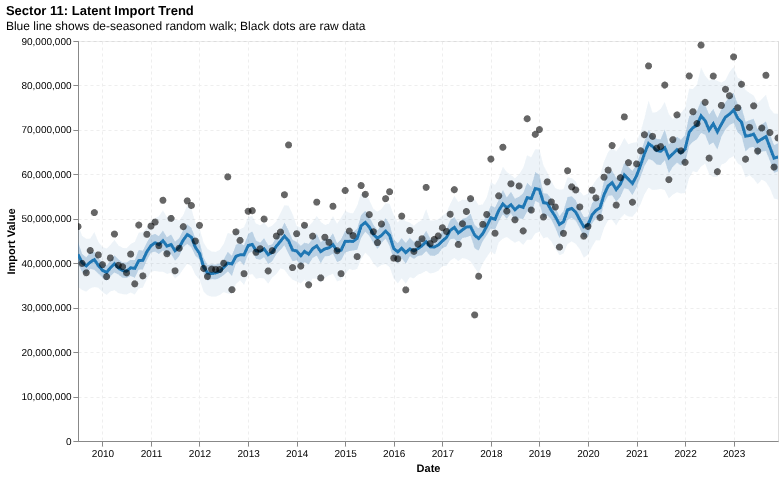
\includegraphics[width=1\linewidth]{assets/visualization.png}
	\end{tikzfigure}

	\begin{center}
		\begin{tabular}{l c c c}
			\hline
			\textbf{Estadístico} & \textbf{Capital ($K$)} & \textbf{Trabajo ($L$)} & \textbf{Energía ($E$)} \\
			\hline
			Promedio (Media)     & $3.50 \times 10^9$     & 14956.25               & $1.73 \times 10^7$     \\
			Desv. Estándar       & $1.05 \times 10^9$     & 47974.77               & $3.04 \times 10^7$     \\
			Mínimo               & $6.03 \times 10^7$     & 330.00                 & $-1.54 \times 10^7$    \\
			\hline
			Percentil 25\%       & $3.47 \times 10^9$     & 2669.75                & $4.90 \times 10^6$     \\
			Mediana (50\%)       & $3.81 \times 10^9$     & 4499.00                & $8.63 \times 10^6$     \\
			Percentil 75\%       & $4.18 \times 10^9$     & 9527.25                & $1.74 \times 10^7$     \\
			Máximo               & $4.67 \times 10^9$     & 434890.00              & $2.88 \times 10^8$     \\
			\hline
		\end{tabular}
	\end{center}
	\vspace{1em}
	\small \textit{Nota: Capital y Energía se presentan en niveles sintéticos antes de la transformación logarítmica.}
}


	% --- COLUMN 3: Analysis ---
	\column{0.25}
	\block{Modelo}{
	Para esta investigación se implemento una función de producción Cobb-Douglas espacio-temporal
	en forma log-lineal para evaluar la resiliencia y el crecimiento diferenciado a nivel municipal
	en Puerto Rico (2021-2024).

	\vspace{0.5em}
	El modelo asume una distribución Normal para las observaciones de energía ($\log y$):
	\begin{equation}
		\log(y_{i,j}) \sim \text{Normal}(\mu_{i,j}, \sigma_{\epsilon})
	\end{equation}
	Donde el valor esperado para el municipio $j$ en el tiempo $i$ se define como:
	\begin{equation}
		\mu_{i,j} = \alpha_j + \lambda_j t_i + \beta_{k,j} \log(k_{i,j}) + \beta_{l,j} \log(l_{i,j}) + \phi(t_i)
	\end{equation}

	\vspace{0.5em}
	Las elasticidades de capital ($\beta_k$) y trabajo ($\beta_l$) comparten fuerza estadística a través de una
	estructura jerárquica con priors informativos centrados en valores teóricos \cite{gordon2016rise}:
	\begin{itemize}[leftmargin=1.5em]
		\item $\beta_{k,j} \sim \text{Normal}(\mu_{\beta_k}, 0.05)$ con $\mu_{\beta_k} \approx 0.3$
		\item $\beta_{l,j} \sim \text{Normal}(\mu_{\beta_l}, 0.05)$ con $\mu_{\beta_l} \approx 0.7$
	\end{itemize}

	\vspace{0.5em}
	El componente temporal se descompone en dos capas críticas:
	\begin{itemize}[leftmargin=1.5em]
		\item \textbf{Tendencias Independientes ($\lambda_j$):} Las pendientes (\texttt{muni\_slope}) no son jerárquicas ($\sigma = 0.1$). Esto permite identificar "ganadores y perdedores" genuinos, evitando que las tendencias locales regresen a la media global.
		\item \textbf{Componente Macro ($\phi(t)$):} Un Proceso Gaussiano en el Espacio de Hilbert (\textbf{HSGP}) captura choques sistémicos de la isla (inflación, cambios en la red eléctrica) mediante $m=20$ funciones de base.
	\end{itemize}
}

	\block{Resultados: Elasticidades y Dinámica de Crecimiento}{
	Los resultados del modelo revelan la estructura de producción agregada y la heterogeneidad en el crecimiento de la Productividad Total de los Factores (TFP) a nivel municipal.

	\vspace{0.5em}
	Las elasticidades estimadas muestran una alta intensidad de mano de obra en la producción, consistente con la economía de servicios y manufactura ligera de la región. El parámetro $\eta_{gp}$ sugiere una volatilidad macroeconómica moderada capturada por el HSGP.

	\begin{center}
		\begin{tabular}{l c c c c}
			\hline
			\textbf{VAR}                     & \textbf{Media} & \textbf{STD} & \textbf{HDI 3\%} & \textbf{HDI 97\%} \\
			\hline
			Elasti Capital ($\mu_{\beta_k}$) & 0.306          & 0.057        & 0.193            & 0.407             \\
			Elasti Trabajo ($\mu_{\beta_l}$) & 0.707          & 0.047        & 0.615            & 0.790             \\
			Amplitud GP ($\eta_{gp}$)        & 0.079          & 0.060        & 0.000            & 0.185             \\
			\hline
		\end{tabular}
	\end{center}

	\vspace{0.5em}
	El modelo identifica variaciones sutiles pero divergentes en las tendencias de crecimiento a largo plazo ($\lambda_j$).
}


	% --- COLUMN 4: Discussion & Closing ---
	\column{0.25}
	\block{}{
	\begin{itemize}[leftmargin=1.5em]
		\item \textbf{Líderes de Crecimiento:} Juana Díaz, Carolina y Manatí encabezan la lista con tendencias positivas ($\approx 0.002$), sugiriendo una expansión en la eficiencia de uso de energía relativa a sus insumos de capital y trabajo.
		\item \textbf{Zonas de Declive:} Cidra, Aguada y Canóvanas muestran las tendencias más bajas ($\approx -0.003$), lo que podría indicar estancamiento industrial o procesos de deseconomía de escala en el periodo 2021-2024.
	\end{itemize}

	\begin{tikzfigure}[Estimacion de importaciones del sector 11]
		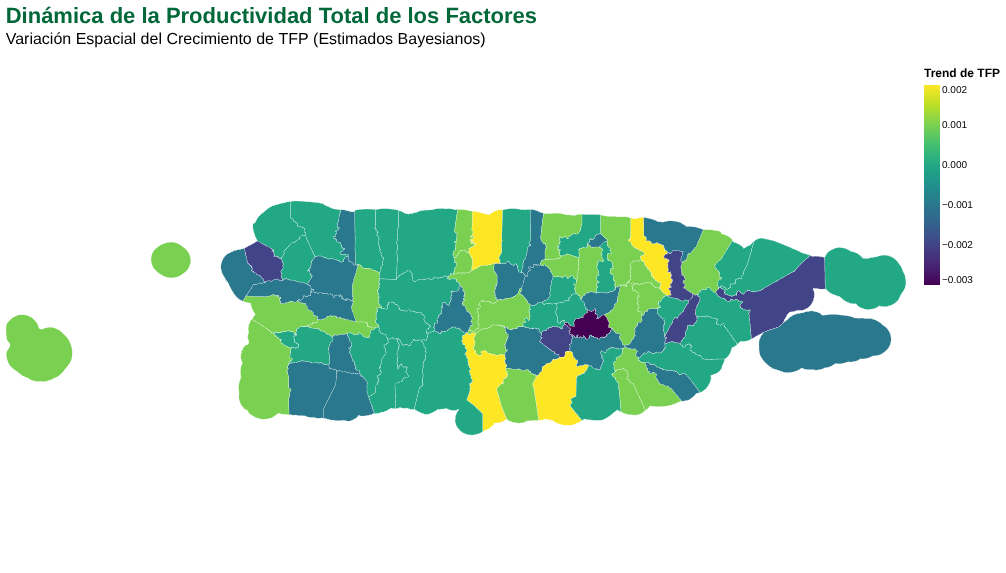
\includegraphics[width=1\linewidth]{assets/maps.png}
	\end{tikzfigure}
}



	\block{Conclusión}{
	Este estudio presenta una contribución importante al análisis de la economía regional de Puerto Rico al
	proponer un marco metodológico capaz de mitigar la histórica escasez de datos macroeconómicos a nivel municipal.
	A través estudio, se logró modelar de manera robusta la función de producción Cobb-Douglas
	para los 78 municipios de la isla durante el periodo 2021-2024.

	\vspace{0.5em}
	En conclusión, aunque el uso de indicadores sintéticos y probabilísticos abre una ventana crucial para entender
	las asimetrías económicas internas de Puerto Rico, se hace evidente la necesidad urgente de institucionalizar
	la recolección de datos de inversión y cuentas de producción municipales. Futuras extensiones de este trabajo
	se enfocarán en refinar el modelo de capital sintético incorporando variables espaciales explícitas (matrices
	de adyacencia municipal) para capturar efectos de desbordamiento (\textit{spillovers}) entre regiones vecinas.
}


	\block{References}{
	\vspace{-0.5em}
	\begin{footnotesize}
		\printbibliography[heading=none]
	\end{footnotesize}
}

\end{columns}
\end{document}
